\lecture{3}{12. September 2025}{Fourier Series}

\exercise{1.}
Consider the function $f(x) = \cos x, 0<x<\pi$.

\textit{Hint:} In some cases the expansion can be an even/odd function.

\textit{Hint:} For $m, n \in \mathbb{N}, m \neq n, L > 0$:
\begin{align*}
  \int_{0}^{\frac{\pi}{2}} \cos x \sin(2nx) \, \mathrm{d}x &= - \frac{2n}{1-4n^2} \\
  \int_{0}^{L} \cos \left( \frac{m\pi x}{L} \right) \sin \left( \frac{n \pi x}{L} \right) \, \mathrm{d}x  &= \frac{nL}{\pi \left( m^2 - n^2 \right)} \left( \cos \left( n\pi \right) \cos(m\pi) -1\right) \\
  \int_{0}^{L} \cos \left( \frac{\pi x}{L} \right) \sin \left( \frac{\pi x}{L} \right) \, \mathrm{d}x &= 0
.\end{align*}

\paragraph{(a)} Sketch the expansion of $f$ and find the corresponding Fourier series.
\bigbreak
The expansion of $f$ is simply the ``repetition'' of $f$ indefinitely along the $x$-axis. This is shown on \autoref{fig:e3_1}
\begin{figure} [ht]
  \centering
  
\includegraphics[width=0.8\linewidth]{./figures/e3_1.png}
  \caption{Expansion of $f(x) = \cos x, 0<x<\pi$}
  \label{fig:e3_1}
\end{figure}

To find the Fourier series of this we must first define a periodic function $f_0(x)$ around $x = 0$ based on \autoref{fig:e3_1} we see that this can be written as
\begin{align*}
  f_0(x) &= \begin{cases}
  \cos x, & 0 < x <\frac{\pi}{2}\\
  - \cos x, & - \frac{\pi}{2} < x < 0
  .\end{cases} \\
    f_0(x) &= f_0(x+p), p = 2L = \pi
.\end{align*}
As $f_0(x)$ is an odd function its Fourier series will be a so-called Fourier sine series:
\[ 
f(x) = \sum_{n = 1}^{\infty} b_n \sin \left( \frac{n\pi x}{L} \right)
.\]
Where the Fourier coefficient $b_n$ is
\[ 
b_n = \frac{2}{L} \int_{0}^{L} f(x) \sin \left( \frac{n \pi x}{L} \right) \, \mathrm{d}x 
.\]
Substituting the general $f(x)$ for our $f_0(x)$ we get:
\begin{align*}
  b_n &= \frac{4}{\pi} \int_{0}^{\frac{\pi}{2}} \cos x \sin \left( 2n x \right) \, \mathrm{d}x  \\
      &= \frac{4}{\pi} \cdot \left( -\frac{2n}{1 - 4n^2} \right) \\
      &= \frac{8n}{\pi \left( 4 n^2 - 1 \right)}
.\end{align*}
Hence the Fourier series becomes:
\[ 
f_0(x) = \sum_{n = 1}^{\infty} \frac{8n}{\pi \left( 4n^2 - 1 \right)} \sin (2n x)
.\]

\paragraph{(b)} Sketch the even expansion of $f$ and find the corresponding Fourier cosine series.
\bigbreak
\begin{figure} [ht]
  \centering
  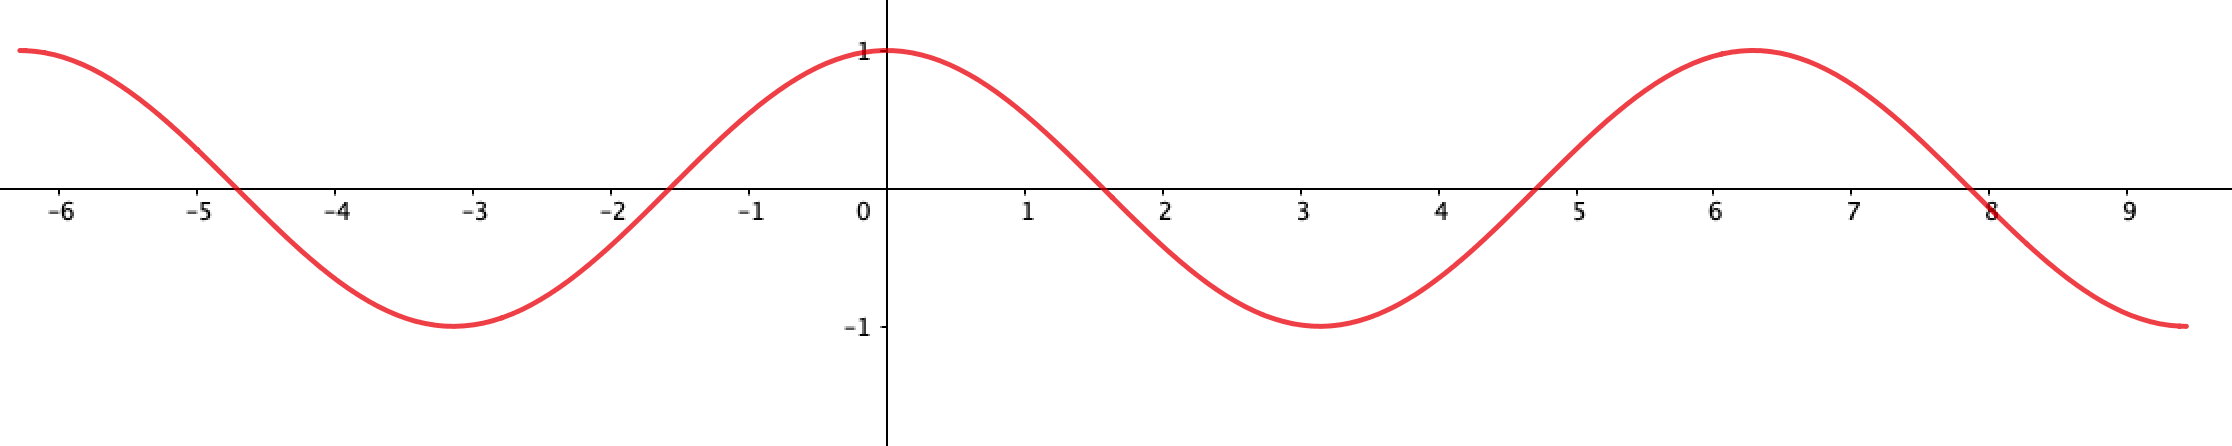
\includegraphics[width=0.8\linewidth]{./figures/e3_1a.png}
  \caption{Even expansion of $f(x) = \cos x, 0 < x < \pi$}
  \label{fig:e3_1a}
\end{figure}
On \autoref{fig:e3_1a} it can be seen that the even expansion of the expression is simply the $\cos$ function. We can therefore write our periodic function as
\begin{align*}
  f_1(x) &= \cos x, \quad 0 < x < \frac{\pi}{2} \\
  f_1(x) &= f_1(x + p), \quad p = 2L = 2\pi
.\end{align*}
This can also be written as
\[ 
f_1 (x) = \cos x
.\]
We remember that the general form of a Fourier cosine series is
\[ 
f(x) = a_0 + \sum_{n = 1}^{\infty} a_n \cos \left( \frac{n \pi x}{L} \right)
\]
or with the values given in the exercise
\[ 
f_1(x) = a_0 + \sum_{n = 1}^{\infty} a_n \cos \left( \frac{n \pi x}{\pi} \right) = a_0 + \sum_{n = 1}^{\infty} a_n \cos nx
.\]
Now we can compare these
\begin{gather*}
  \cos x = a_0 + \sum_{n = 1}^{\infty} a_n \cos nx \\
  \implies a_0 = 0, a_1 = 1
.\end{gather*}


\paragraph{(c)} Sketch the odd expansion of $f$ and find the corresponding Fourier sine series.
\begin{figure} [ht]
  \centering
  
\includegraphics[width=0.5\linewidth]{./figures/e3_1.png}
  \caption{Odd expansion of $f(x) = \cos x, 0 < x < \pi$}
\end{figure}
The odd expansion gives the periodic function
\begin{align*}
  f_2(x) &= \begin{cases}
  \cos x, & 0 < x < \pi\\
  - \cos x & -\pi < x < 0
  .\end{cases}\\
    f_2(x) &= f_2(x+p), \quad p = 2L = 2\pi
.\end{align*}
We remember that the general form of a Fourier sine series is
\[ 
f(x) = \sum_{n = 1}^{\infty} b_n \sin \left( \frac{n\pi x}{L} \right)
\]
or with the values in the exercise
\[ 
f_2(x) = \sum_{n = 1}^{\infty} b_n \sin \left( nx \right)
\]
where $b_n$ is
\[ 
b_n = \frac{2}{L} \int_{0}^{L} f(x) \sin \left( \frac{n \pi x}{L} \right) \, \mathrm{d}x  
\]
or
\[ 
b_n = \frac{2}{\pi} \int_{0}^{\pi} \cos x \sin \left( n x \right) \, \mathrm{d}x 
.\]
For $n = 1$ this simplifies to
\[ 
b_1 = 0
.\]
For $n > 1$ it becomes
\begin{align*}
  b_n &= \frac{2}{\pi} \cdot \frac{n \pi}{\pi \left( 1 - n^2 \right)} \left(- \cos (n \pi)  - 1 \right) \\
  &= \frac{2n}{\pi \left( n^2 - 1 \right)} \left( 1 - \cos \left( n \pi \right) \right)
.\end{align*}
Hence the full Fourier sine series is
\[ 
f_2(x) = \sum_{n = 2}^{\infty} \frac{2n}{\pi \left( n^2 - 1 \right)} \left( 1 + \cos \left( n\pi \right) \right) \sin \left( nx \right)
.\]


\paragraph{(d)} Calculate the error $E_N$ of the expansion and the odd expansion for $N = 1,2,3$. What can be said about the quality of the approximations for these two expansions?
\bigbreak
The general formula for calculating the error $E_N$ of the approximation is
\[ 
E_N = \int_{-L}^{L} f^2(x) \, \mathrm{d}x - L \left( 2a_0^2 + \sum_{n = 1}^{N} \left( a_n^2 + b_n^2 \right) \right)
.\]
If we start by considering the \textit{expansion} we are working with the expression
\[ 
  f_0(x) = \sum_{n= 1}^{\infty} \frac{8n}{\pi \left( 4n^2 - 1 \right)} \sin \left( 2nx \right)
.\]
Over the entire interval $[-L; L]$ $f_0^2 = \cos^2$. Using this fact and substituting $L = \frac{\pi}{2}$, $a_n = 0$ and $b_n = \frac{8n}{\pi \left( 4n^2 - 1 \right)}$ we can write
\begin{align*}
  E_N &= \int_{- \frac{\pi}{2}}^{\frac{\pi}{2}} \cos^2(x) \, \mathrm{d}x - \frac{\pi}{2} \sum_{n = 1}^{N} \left( \frac{8n}{\pi \left( 4n^2 -1 \right)} \right)^2 \\
  &= \int_{-\frac{\pi}{2}}^{\frac{\pi}{2}}  \frac{1}{2} \left( 1 + \cos (2x) \right) \, \mathrm{d}x - \frac{\pi}{2} \sum_{n = 1}^{N} \frac{64n^2}{\pi^2 \left( 4n^2 - 1 \right)^2} \\
  &= \frac{\pi}{2} + \frac{1}{2} \left[ \frac{1}{2} \sin \left( 2x \right) \right]_{- \frac{\pi}{2}}^{\frac{\pi}{2}} - \frac{32}{\pi} \sum_{n = 1}^{N} \frac{n^2}{\left( 4n^2 - 1 \right)^2} \\
  &= \frac{\pi}{2} - \frac{32}{\pi} \sum_{n = 1}^{N} \frac{n^2}{\left( 4n^2 - 1 \right)^2}
.\end{align*}
Calculating the numerical value of this for $n = 1,2,3$ yields
\begin{align*}
  E_1 &= \frac{\pi}{2} - \frac{32}{9\pi} \approx \num{0,439} \\
  E_2 &= \frac{\pi}{2} - \frac{32}{\pi} \left( \frac{1}{9} + \frac{4}{15^2} \right) \approx \num{0,258} \\
  E_3 &= \frac{\pi}{2} - \frac{32}{\pi} \left( \frac{1}{9} + \frac{4}{15^2} + \frac{9}{35^2} \right) \approx \num{0,183} 
.\end{align*}

Now moving on to the odd expansion our $f_2^2(x) = \cos^2(x)$ as before, however this time $L = \pi$ and $b_n = \frac{2n}{\pi \left( n^2 - 1 \right)} \left( 1 + \cos \left( n\pi \right) \right)$. Plugging these values into the formula we get:
\begin{align*}
  E_N &= \int_{-\pi}^{\pi} \cos^2(x) \, \mathrm{d}x - \pi \sum_{n = 2}^{N} \left( \frac{2n}{\pi \left( n^2 - 1 \right)} \left( 1 + \cos \left( n \pi \right) \right) \right)^2 \\
  &= \pi - \pi \sum_{n = 2}^{N} \frac{4n^2}{\pi^2 \left( n^2 - 1 \right)^2} \left( 1 + \cos \left( n\pi \right) \right)^2 \\
  &= \pi - \frac{4}{\pi} \sum_{n = 2}^{N} \frac{n^2}{\left( n^2 - 1 \right)^2} \left( 1 + \cos(n \pi) \right)^2
.\end{align*}
And for $n = 1,2,3$ we get
\begin{align*}
  E_1 &= \pi - \frac{4}{\pi}\cdot 0 = \pi \\
  E_2 &= \pi - \frac{4}{\pi} \left( 0 + \frac{16}{9} \right) \approx \num{0,878}  \\
  E_3 &= \pi - \frac{4}{\pi } \left( 0 + \frac{16}{9} + \frac{9}{64} \cdot 0 \right) \approx \num{0,878} 
.\end{align*}

When comparing errors we must take into account the length of the intervals $L$. Therefore a realistic comparison requires us to half the errors from the odd expansion. Even when doing so the error rate from the ``normal'' expansion performs better and should therefore be preferred.

\exercise{2.}
Find the Fourier integral representation of
\[ 
f(x) = \begin{cases}
  1, & -1 < x < 1 \\
  -1, & 1 < x < 2 \\
  -1, & -2 < x < -1 \\
   0, & \text{otherwise}
.\end{cases}
.\]
\bigbreak
The Fourier integral is given by
\[ 
f(x) = \int_{0}^{\infty} \left( A (\omega) \cos (\omega x) + B(\omega) \sin(\omega x) \right) \, \mathrm{d}\omega
\]
where
\[ 
A (\omega) = \frac{1}{\pi} \int_{-\infty}^{\infty} f(x) \cos(\omega x) \, \mathrm{d}x 
\]
and
\[ 
B(\omega) = \frac{1}{\pi} \int_{-\infty}^{\infty} f(x) \sin \left( \omega x \right) \, \mathrm{d}x 
.\]
We start by finding $A(\omega)$ using piecewise integration
\begin{align*}
  A(\omega) &= \frac{1}{\pi} \left( \int_{-2}^{-1} - \cos \left( \omega x \right) \, \mathrm{d}x  + \int_{-1}^{1} \cos (\omega x) \, \mathrm{d}x + \int_{1}^{2} - \cos(\omega x) \, \mathrm{d}x \right) \\
            &= \frac{4 \sin \omega - 2 \sin (2\omega)}{\pi \omega}
.\end{align*}
The same technique can now be applied to find $B (\omega)$ as
\begin{align*}
  B(\omega) &= \frac{1}{\pi} \left( \int_{-2}^{-1} - \sin (\omega x) \, \mathrm{d}x  + \int_{-1}^{1} \sin (\omega x) \, \mathrm{d}x  + \int_{1}^{2} - \sin(\omega x) \, \mathrm{d}x  \right) \\
            &= 0
.\end{align*}
Therefore the Fourier integral representation of $f(x)$ is
\[ 
f(x) = \int_{0}^{\infty} \left( \frac{4 \sin \omega - 2 \sin (2\omega)}{\pi \omega} \right) \cos (\omega x) \, \mathrm{d}\omega
.\]

\exercise{3.}
Find the Fourier integral representation of
\[ 
f(x) = \begin{cases}
-1, & -2 < x < 0\\
1,  & 0 < x < 2 \\
0, & \text{otherwise}
.\end{cases}
.\]
\bigbreak
Here the same procedure can be applied as above to get
\begin{align*}
  A(\omega) &= \frac{1}{\pi} \left( \int_{-2}^{0} - \cos(\omega x) \, \mathrm{d}x  + \int_{0}^{2} \cos (\omega x) \, \mathrm{d}x  \right) \\
            &= 0
.\end{align*}
and
\begin{align*}
  B(\omega) &= \frac{1}{\pi} \left( \int_{-2}^{0} - \sin(\omega x) \, \mathrm{d}x  + \int_{0}^{2} \sin (\omega x) \, \mathrm{d}x  \right) \\
            &= \frac{2 - 2 \cos (2\omega)}{\pi \omega}
.\end{align*}
Which becomes
\[ 
f(x) = \int_{0}^{\infty} \frac{2 - 2 \cos (2\omega)}{\pi \omega} \sin (\omega x) \, \mathrm{d}\omega
.\]


\exercise{4.}
Consider the periodic rectangular wave and its Fourier series as discussed in Lecture 1. Calculate the error of the $N$-th approximation for $N = 1,2,3$.
\bigbreak
The general formula for calculating the error $E_N$ of the approximation is
\[ 
E_N = \int_{-L}^{L} f^2(x) \, \mathrm{d}x - L \left( 2a_0^2 + \sum_{n = 1}^{N} \left( a_n^2 + b_n^2 \right) \right)
.\]
In this case $f(x)^2 = k^2$, $L = \pi$, $a_0 = 0$, $a_n = 0$, and $b_n = \frac{2k}{n\pi} \left( 1 - \cos(n\pi) \right)$. I.e.
\begin{align*}
  E_N &= \int_{-\pi}^{\pi} k^2 \, \mathrm{d}x - \pi \sum_{n = 1}^{\infty} \left( \frac{2k}{n\pi} \left( 1 - \cos \left( n\pi \right) \right)\right)^2 \\
      &= 2\pi k^2 - \frac{4k^2}{\pi} \sum_{n = 1}^{N} \frac{1}{n^2} \left( 1 - \cos(n \pi) \right)^2
.\end{align*}
For $n = 1,2,3$ we get $E_1 = E_2 \approx \num{1,19} k^2$ and $E_3 \approx \num{0,62} k^2$.

